\documentclass[10pt,aspectratio=169,serif,fleqn]{beamer}

\usepackage[fontset=none, scheme=plain]{ctex}
\IfFontExistsTF{Songti SC}{%
	\setCJKmainfont{Songti SC}[AutoFakeSlant=0.2]%
	\setCJKsansfont{Songti SC}[AutoFakeSlant=0.2]%
}{%
	\setCJKmainfont{FandolSong-Regular}[Extension=.otf,BoldFont=FandolSong-Bold,AutoFakeSlant=0.2]%
	\setCJKsansfont{FandolSong-Regular}[Extension=.otf,BoldFont=FandolSong-Bold]%
}
\usepackage{amsmath,amssymb,graphicx,tikz,booktabs,multicol,calligra}
\usepackage{pgfplots}
\pgfplotsset{compat=1.18}
\usepackage{tcolorbox}
\tcbuselibrary{skins}
\usepackage{XyygU}
\usepackage{caption}
\captionsetup[figure]{name=图,labelsep=period}

\usetikzlibrary{arrows.meta,positioning,calc}

\setlength{\abovedisplayskip}{0pt plus 2pt minus 2pt}
\setlength{\belowdisplayskip}{0pt plus 2pt minus 2pt}

\title[习题3.3]{P91 练习及习题3.3 }
\subtitle{}
\author{}
\institute{}
\date{2026-10-28}

\begin{document}

\begin{frame}
  \titlepage
\end{frame}

% ========== 第1题 ==========
\begin{frame}[t]{练习 \textbf{1.} 已知幂函数 $y=f(x)$ 的图象过点 $(2,\sqrt{2})$，求这个函数的解析式。}
	
	\vspace{-2em}
		\begin{tcolorbox}[colback=orange!10,colframe=orange,title=\textbf{解}]
		设幂函数为 $f(x)=x^{\alpha}$。
		
		\vspace{0.3em}
		因其图象过点 $(2,\sqrt{2})$，代入得：
		\[
		2^{\alpha}=\sqrt{2}=2^{\frac12},
		\]
		所以 $\alpha=\dfrac12$。
		
		\vspace{0.5em}
		故所求函数解析式为
		\[
		\alert{f(x)=x^{\frac12}=\sqrt{x}},\quad x\ge 0.
		\]
	\end{tcolorbox}
\end{frame}



% ========== 第2题 ==========
\begin{frame}[t]{练习 \textbf{2.} 利用幂函数的性质，比较下列各题中两个值的大小：}
	
	
	\vspace{-1em}
	(1) $(-1.5)^3$，$(-1.4)^3$；
	
	\vspace{0.5em}
	(2) $\dfrac{1}{-1.5}$，$\dfrac{1}{-1.4}$。
	
	
		\begin{tcolorbox}[colback=orange!10,colframe=orange,title=\textbf{解}]
		(1) 幂函数 $y=x^3$ 在 $\mathbf{R}$ 上单调递增。
		
		\vspace{0.3em}
		因为 $-1.5<-1.4$，所以 $(-1.5)^3\alert{<}(-1.4)^3$。
		
		\vspace{0.8em}
		(2) $\dfrac{1}{-1.5}=(-1.5)^{-1}$，$\dfrac{1}{-1.4}=(-1.4)^{-1}$。
		
		\vspace{0.3em}
		幂函数 $y=x^{-1}$ 在 $(-\infty,0)$ 上单调递减。
		
		\vspace{0.3em}
		因为 $-1.5<-1.4$，所以 $(-1.5)^{-1}\alert{>}(-1.4)^{-1}$，
		即 $\dfrac{1}{-1.5}>\dfrac{1}{-1.4}$。
	\end{tcolorbox}
\end{frame}


% ========== 第3题 ==========
\begin{frame}[t]{练习 \textbf{3.} 根据单调性和奇偶性的定义，讨论函数 $f(x)=x^3$ 的单调性，并判断其奇偶性。}
	\vspace{-1.6em}
	\begin{tcolorbox}[colback=orange!10,colframe=orange,title=\textbf{解}]
		\textbf{奇偶性：} 定义域为 $\mathbf{R}$，关于原点对称。
		\[
		f(-x)=(-x)^3=-x^3=-f(x),
		\]
		故 $f(x)=x^3$ 是 \alert{奇函数}。
		
		\vspace{0.8em}
		\textbf{单调性：} 任取 $x_1<x_2$，
		\[
		f(x_1)-f(x_2)=x_1^3-x_2^3=(x_1-x_2)(x_1^2+x_1x_2+x_2^2).
		\]
		因 $x_1-x_2<0$，而 $x_1^2+x_1x_2+x_2^2=\left(x_1+\dfrac{x_2}{2}\right)^2+\dfrac34x_2^2>0$（仅 $x_1=x_2=0$ 时取等），
		
		\vspace{0.3em}
		故 $f(x_1)-f(x_2)<0$，即 $f(x_1)<f(x_2)$，$f(x)=x^3$ 在 $\mathbf{R}$ 上 \alert{单调递增}。
	\end{tcolorbox}
\end{frame}


\begin{frame}[t]{第3题 图象}
	\begin{center}
		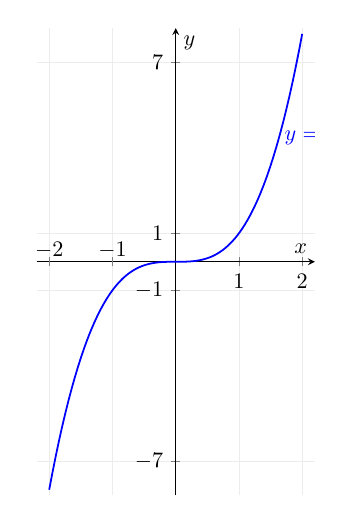
\begin{tikzpicture}[scale=0.8]
			\begin{axis}[
%				axis equal,
				width=6cm, height=9cm,
				axis lines=middle,
				xlabel=$x$, ylabel=$y$,
				xmin=-2.2, xmax=2.2, ymin=-8.2, ymax=8.2,
				xtick={0,1,2},
				extra x ticks={-1,-2},
				extra x tick style={x tick label style={above}},
				ytick={-7,-1,0,1,7},
				grid=major, grid style={gray!15},
				]
				\addplot[thick,blue,domain=-2:2,samples=80] {x^3};
				\node[blue,right] at (axis cs:1.6,4.5) {$y=x^3$};
			\end{axis}
		\end{tikzpicture}
	\end{center}
\end{frame}








% ========== 第1题 ==========
\begin{frame}[t]{习题 \textbf{1.} 画出函数 $y=\sqrt{|x|}$ 的图象，并判断函数的奇偶性，讨论函数的单调性。}


\begin{tcolorbox}[colback=orange!10,colframe=orange,title=\textbf{解}]
	\[
	y=\sqrt{|x|}=\begin{cases}\sqrt{x}, & x\ge 0,\\ \sqrt{-x}, & x<0.\end{cases}
	\]
	\textbf{奇偶性：} 定义域 $\mathbf{R}$，$f(-x)=\sqrt{|-x|}=\sqrt{|x|}=f(x)$，故为 \alert{偶函数}。
	
	\vspace{0.5em}
	\textbf{单调性：} 当 $x\ge0$ 时 $y=\sqrt{x}$ 单调递增；由偶函数对称性，$x<0$ 时单调递减。
	
	\vspace{0.3em}
	单调递减区间：$(-\infty,0]$；单调递增区间：$[0,+\infty)$。
\end{tcolorbox}
\end{frame}



\begin{frame}[t]{第1题 图象}
\begin{center}
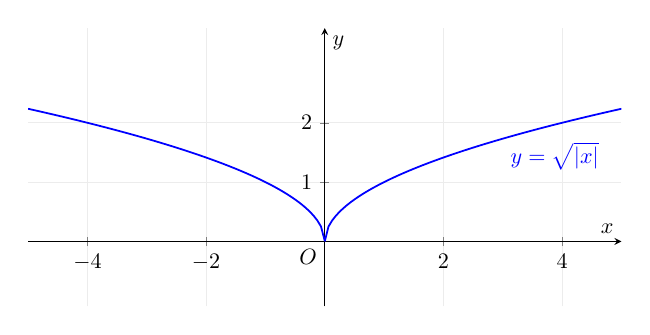
\begin{tikzpicture}[scale=0.8]
\begin{axis}[
	axis equal,
    width=11cm, height=6cm,
    axis lines=middle,
    xlabel=$x$, ylabel=$y$,
    xmin=-5, xmax=5, ymin=0, ymax=2.5,
    xtick={-4,-2,0,2,4},
    ytick={1,2},
    grid=major, grid style={gray!15},
]
\addplot[thick,blue,domain=0:5,samples=80] {sqrt(x)};
\addplot[thick,blue,domain=-5:0,samples=80] {sqrt(-x)};
\node[blue,below right] at (axis cs:3,1.8) {$y=\sqrt{|x|}$};
\node[below left] at (0,0) {$O$};
\end{axis}
\end{tikzpicture}
\end{center}
\end{frame}

% ========== 第2题 ==========
\begin{frame}[t]{第2题：气体流量与管道半径}
\textbf{2.} 在固定压力差下，当气体通过圆形管道时，其流量 $v$（单位：cm$^3$/s）与管道半径 $r$（单位：cm）的四次方成正比。

(1) 写出气体流量 $v$ 关于管道半径 $r$ 的函数解析式；

(2) 若气体在半径为 $3$ cm 的管道中，流量为 $400$ cm$^3$/s，求该气体通过半径为 $r$ 的管道时，其流量 $v$ 的表达式；

(3) 已知(2)中的气体通过的管道半径为 $5$ cm，计算该气体的流量（精确到 $1$ cm$^3$/s）。
\end{frame}

\begin{frame}[t]{}\vspace{-1em}
\begin{tcolorbox}[colback=orange!10,colframe=orange,title=\textbf{解}]
(1) 由题意 $v=kr^4$（$k>0$ 为比例系数）。

\vspace{0.5em}
(2) 代入 $r=3$，$v=400$：
\[
400=k\cdot 3^4=81k,\quad k=\frac{400}{81}.
\]
故
\[
v=\frac{400}{81}r^4.
\]

\vspace{0.5em}
(3) 当 $r=5$ 时：
\[
v=\frac{400}{81}\cdot 5^4=\frac{400\times 625}{81}=\frac{250000}{81}\approx 3086\ \text{cm}^3/\text{s}.
\]
\end{tcolorbox}
\end{frame}

% ========== 第3题 ==========
\begin{frame}[t]{\textbf{3.} 试用描点法画出函数 $f(x)=x^{-2}$ 的图象，求函数的定义域、值域；讨论函数的单调性、奇偶性，并证明。}
	\vspace{-2em}
\begin{tcolorbox}[colback=orange!10,colframe=orange,title=\textbf{解}]
	$f(x)=x^{-2}=\dfrac{1}{x^2}$。
	
	\vspace{0.3em}
	\textbf{定义域：} $(-\infty,0)\cup(0,+\infty)$；
	
	\textbf{值域：} $(0,+\infty)$（$x^2>0$ 且可取任意正数）。
	
	\vspace{0.5em}
	\textbf{奇偶性：} $f(-x)=\dfrac{1}{(-x)^2}=\dfrac{1}{x^2}=f(x)$，为 \alert{偶函数}。
	
	\vspace{0.5em}
	\textbf{单调性：} 任取 $0<x_1<x_2$，
	\[
	f(x_1)-f(x_2)=\frac1{x_1^2}-\frac1{x_2^2}=\frac{x_2^2-x_1^2}{x_1^2x_2^2}=\frac{(x_2-x_1)(x_2+x_1)}{x_1^2x_2^2}>0,
	\]
	故 $f(x)$ 在 $(0,+\infty)$ 上单调递减；由偶函数对称性，在 $(-\infty,0)$ 上单调递增。
\end{tcolorbox}
\end{frame}



\begin{frame}[t]{第3题 图象}
\begin{center}
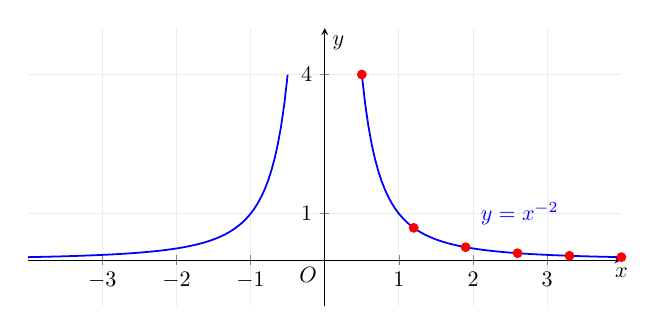
\begin{tikzpicture}[scale=0.8]
\begin{axis}[
    width=11cm, height=6cm,
    axis lines=middle,
    xlabel=$x$, ylabel=$y$,
    xlabel style={below},
    xmin=-4, xmax=4, ymin=-1, ymax=6,
    xtick={-3,-2,-1,1,2,3},
    ytick={1,4},
    grid=major, grid style={gray!15},
    ymax=5,
]
\addplot[thick,blue,domain=0.5:4,samples=80] {1/x^2};
\addplot[samples=6,only marks,,mark options={red},domain=0.5:4]{1/x^2}; 
\addplot[thick,blue,domain=-4:-0.5,samples=80] {1/x^2};
\node[blue,right] at (axis cs:2,1) {$y=x^{-2}$};
\node[below left] at (0,0){$O$};
\end{axis}
\end{tikzpicture}
\end{center}
\end{frame}

\begin{frame}[c]
  \begin{center}
    {\Huge\calligra Thanks!}
  \end{center}
\end{frame}

\end{document}
